\chapter{基于改进Vision Transformer骨髓血细胞检测算法设计与实现}
\section{引言}
% 研究背景,现状 挑战与本文贡献
白血病是一种人体造血系统的恶性肿瘤,在所有恶性肿瘤中占比约5\%,是我国重点防治的十大恶性肿瘤之一。
血细胞形态学检查是白血病诊断常规检查的一部分,各类骨髓血细胞经过染色后呈现出不同的形状、颜色与纹理,
这些细胞由经验丰富的病理专家识别并计数,最终根据FAB标准给出白血病类型的诊断。上述人工镜检的诊断流程存在以下不足,
人工分类计数繁琐费时,诊断结果具有较强的主观性。此外,细胞形态学人才资源紧缺,
培养精通细胞病理诊断的医师要耗费大量的时间。通过研究骨髓血细胞自动化识别技术来辅助临床诊断,可以实现诊断流程的标准化、
快速化与智能化,将医生从繁重的病理工作中解放出来,具有重要的临床意义和广阔的应用前景。

近年来,基于深度学习的方法在医学影像处理领域取得了巨大的成功,
国内外学者纷纷开始探索基于深度学习的血细胞识别方法。基于深度学习的血细胞识别方法不再需要进行复杂的血细胞特征工程
设计,直接将血细胞数据输入网络中进行端到端训练。通过优化损失函数,网络可以自动挖掘数据的潜在特征,并基于这些特征进行
预测,相比于传统识别方法具有更高的识别准确率。根据文献调研,血细胞识别算法主要基于计算机视觉领域的目标识别网络并通过迁移学习进行微调,这些识别
网络包括了ResNext、ResNet与EfficientNet等,在血细胞数据集上获得了很好的识别结果。

骨髓血细胞自动化识别是一项非常具有挑战性的任务,主要存在着以下难点:(1)缺少大规模的骨髓血细胞识别任务数据集,
不同批次的骨髓血细胞存在染色、光照等差异,导致切片图像外观、颜色变化的多样性。
(2)各类骨髓血细胞在人体中的所占比例不同,导致数据集中各个类别样本数量分布不均衡,
数量较少类别的骨髓血细胞难以有效的进行特征学习。
(3)骨髓血细胞种类繁多,例如粒细胞有原始、早幼、中幼与晚幼等阶段,
相邻发育阶段的血细胞在形态上非常类似,骨髓血细胞子类之间差异较小增加了细粒度识别的难度。

针对骨髓血细胞识别过程中的难点,本章提出了一种基于改进Vision Transformer的骨髓血细胞识别方法。
首先,使用第四章提出的改进RetinaNet网络从图像中检测出细胞边界并进行裁剪,去除背景等干扰。
接着,本章提出一种重叠图像块划分方法将裁剪后的图像分割为多个图像块并学习嵌入向量表示。
然后,嵌入向量经过多个编码层进行特征提取。本章基于多头自注意机制提出了稀疏注意力模块,
该模块可以捕捉图像中的辨识性区域,提取图像中的细粒度特征,并将筛选后的特征输入到编码层。
最后,网络输出的分类特征用于骨髓血细胞的识别。在训练过程中,本章采用对比损失进一步增加分类特征的类内一致性与类间差异性。
最后,在邃蓝智能骨髓血细胞数据集与开源的慕尼黑血细胞形态学数据集实验结果表明,
我们提出的方法具有良好的精细分类性能,相比于其他识别方法具有更高的识别准确率

本章内容源自我以第一作者发表的文章《基于改进Vision Transformer的血细胞图像识别方法研究》\cite{SWGC202206005}

\section{改进的Vision Transformer骨髓血细胞识别网络}

本文提出的基于Vision Transformer的骨髓血细胞识别网络框架如图~\ref{fig:vit}所示。
首先将输入的血细胞图像分割为$N$个$P \times P$大小的图像块,接着将图像块线性映射为序列化嵌入向量,
其次加入可学习的分类向量与位置编码信息。然后嵌入向量被输入到多个堆叠的编码模块中进行特征提取。
在最后一层编码模块前,使用辨识性区域选择模块来寻找图像中的区分性像素块并将其对应的隐含特征作为输入。
最后编码器输出的分类特征经过全连接层得到骨髓血细胞的类别概率信息。

\begin{figure} 
   \centering   
   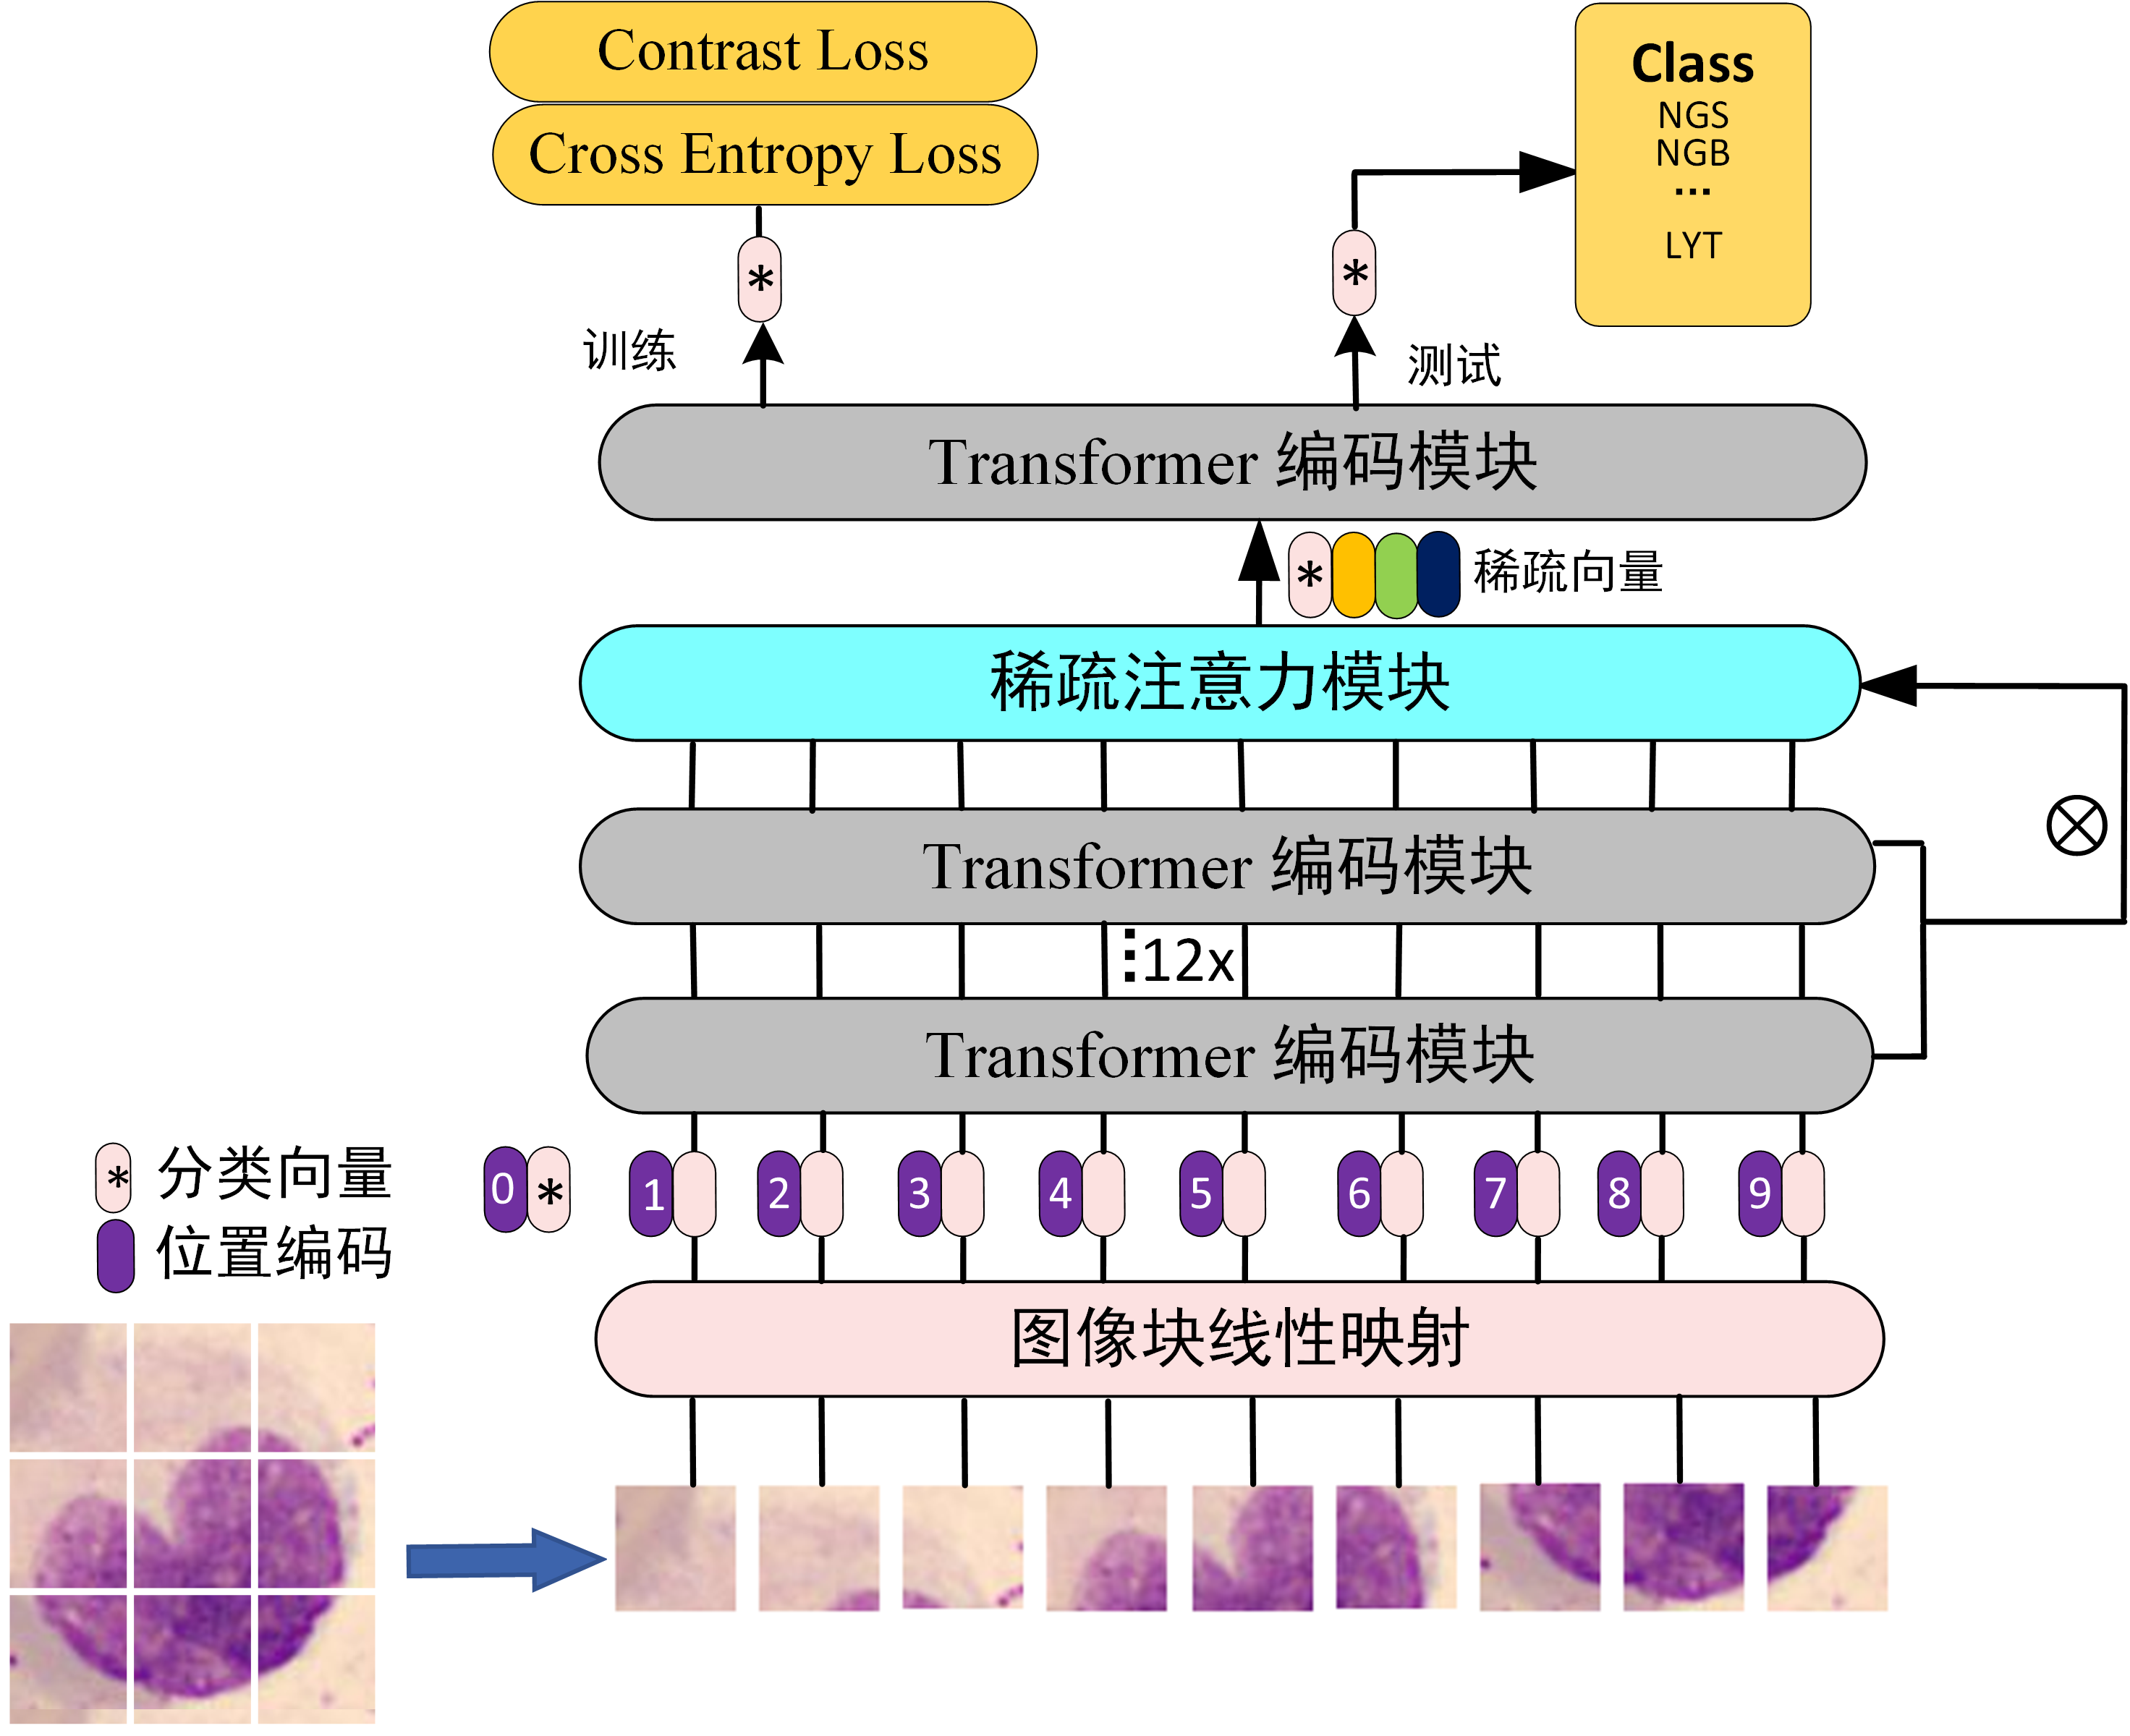
\includegraphics[width=0.9\linewidth]{transFG.png}   
   \caption{基于改进Vision Transformer骨髓血细胞识别网络结构}   
   \label{fig:vit} 
\end{figure}  

\subsection{重叠图像块划分}
Vision Transformer模型接收的输入为序列化数据,因此需要将图像划分为图像块并线性映射为序列化向量(token)。
Vision Transformer模型将图像划分成大小为$P \times P$且互不重叠的像素块,但这样划分会破坏图像的局部结构,
例如辨识性区域被划分到两个相邻的图像块中。为避免该问题,本文采用滑动窗的方法来生成有重叠的图像块。
当输入图像的尺寸为$H \times W \times C$、图像块大小为$P$、滑动窗的步长为$S$时,图像将会被划分为$N$个像素块,
其中$N$如式~\ref{eq:embed}所示。
\begin{equation}
  n=n_{h} \times n_{w}=\left\lfloor\frac{h-p}{s}+1\right\rfloor \times\left\lfloor\frac{w-p}{s}+1\right\rfloor
  \label{eq:embed}
\end{equation}

通过滑动窗的方式,两个相邻像素块的重叠面积为$(P-S) \times P$,更好的保留了图像的局部信息。
当$S$越小,局部结构保存的越完整,但会增加序列化向量的数量导致计算开销变大。
综合利弊,在实验中将S的大小设置为$2P/3$。图像划分完成后,需要将2-D的图像块转化为1-D的序列向量,
首先将图像块展平为一组向量$x_{\mathrm{p}} \in \mathbb{R}^{N \times P^{2} \mathrm{C}}$,
然后通过线性变换将其映射到$D$的维度大小。
上述转化在具体实现上等价于对原图像进行$D$个$P \times P \times P^2C$尺寸的卷积核、步长为$2P/3$的卷积操作。
由于嵌入后的向量不包含位置信息,需要加入一个特殊的可学习位置编码。
此外还加入可学习分类向量作为最终的输出特征用于图像分类。
嵌入后的序列数据$\mathbf{z}_{0}$如式~\ref{eq:embed1}所示,其中$\boldsymbol{E}$为投影矩阵、$\boldsymbol{E}_{\mathrm{pos}}$为位置编码、$\boldsymbol{x}_{\text {class }}$为分类向量。
\begin{equation}
    \mathbf{z}_{0}=\left[\boldsymbol{x}_{\text {class }} ; \boldsymbol{x}_{p}^{1} \boldsymbol{E} ; \boldsymbol{x}_{p}^{2} \boldsymbol{E} ; \cdots ; \boldsymbol{x}_{p}^{N} \boldsymbol{E}\right]+\boldsymbol{E}_{\mathrm{pos}}
    \label{eq:embed1}
\end{equation}

图片序列化之为一组向量后,网络需要知道每一个token在序列中的绝对位置,并且不同token之间的相对位置也需要保持一致。因此引入位置编码(Positional Embedding,PE)来
表示token的位置关系。位置编码采用连续有界的正弦、余弦函数来表示位置信息,受到二进制编码的启发,位置编码向量的低位角频率较大,模拟二进制低位0、1的高频交互,
位置编码高位角频率小,对位置$t$的变动不敏感,模拟二进制的高位变化较小。为了可以用线性变换表示相对位置变动,采用正弦与余弦一组的方式对位置编码进行表示。
定义$t$为这个token在序列中的实际位置,$P E_{t} \in \mathbb{R}^{d}$表示这个token的位置编码向量,$P E_{t}^{(i)}$表示位置编码向量中的第i个
元素,$d_{model}$为位置编码的维度,则位置编码$P E_{t} \in \mathbb{R}^{d}$如式~\ref{eq:pos_embed}所示:
\begin{equation}
  P E_{t}^{(i)}=\left\{\begin{array}{l}
  \sin \left(w_{i} t\right), \quad \text { if } k=2 i \\
  \cos \left(w_{i} t\right), \quad \text { if } k=2 i+1
  \end{array}\right.
  \label{eq:pos_embed}
\end{equation}

其中$w_{i}=\frac{1}{10000^{2 i / d_{\text {model }}}}$,$i=0,1,2,3, \ldots, \frac{d_{\text {model }}}{2}-1$。
token序列长度为50,向量维度为128的位置编码可视化结果如图~\ref{fig:pos_embed}所示。
\begin{figure} 
   \centering   
   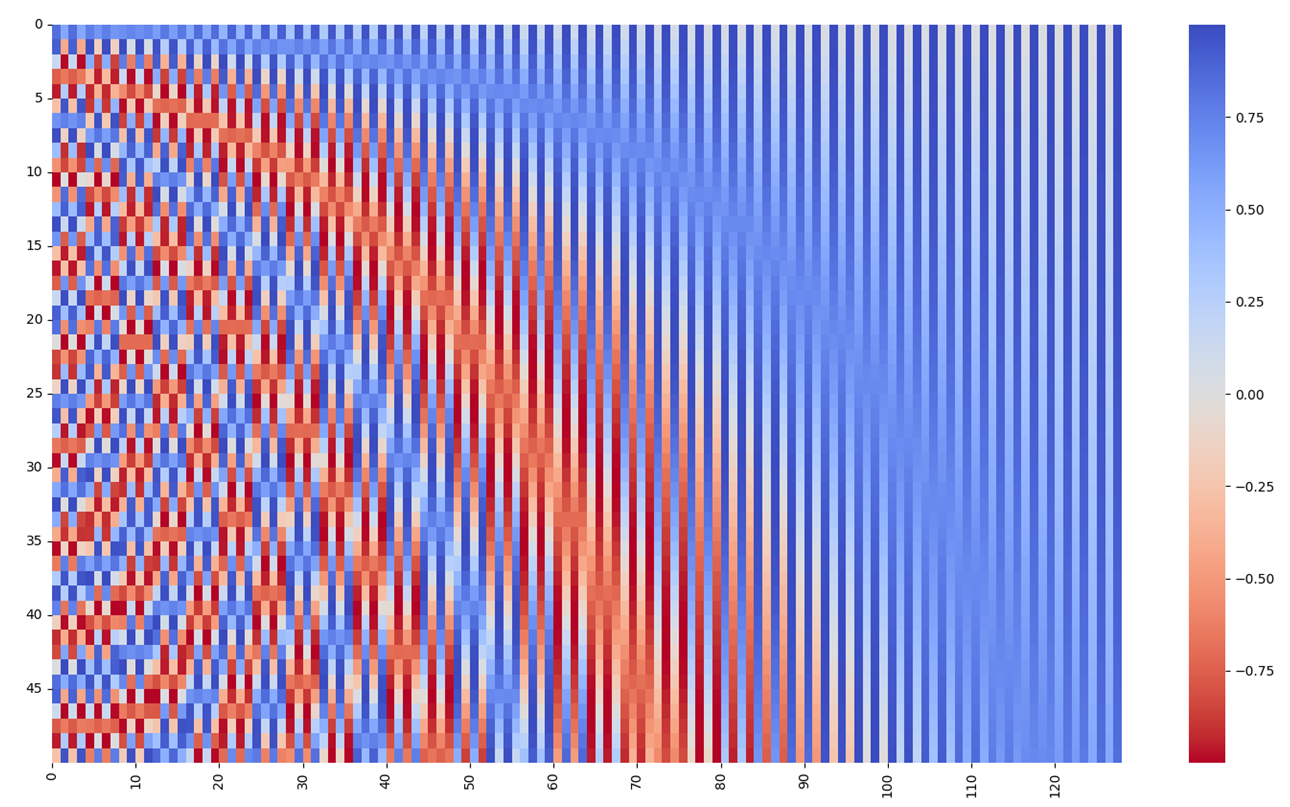
\includegraphics[width=0.80\linewidth]{pos_emb.png}   
   \caption{位置编码可视化}   
   \label{fig:pos_embed} 
\end{figure}  

\subsection{编码层}
Vision Transformer的编码器由$L$个结构相同的编码模块堆叠而成,编码模块结构如图~\ref{fig:encoder}所示:
\begin{figure} 
   \centering   
   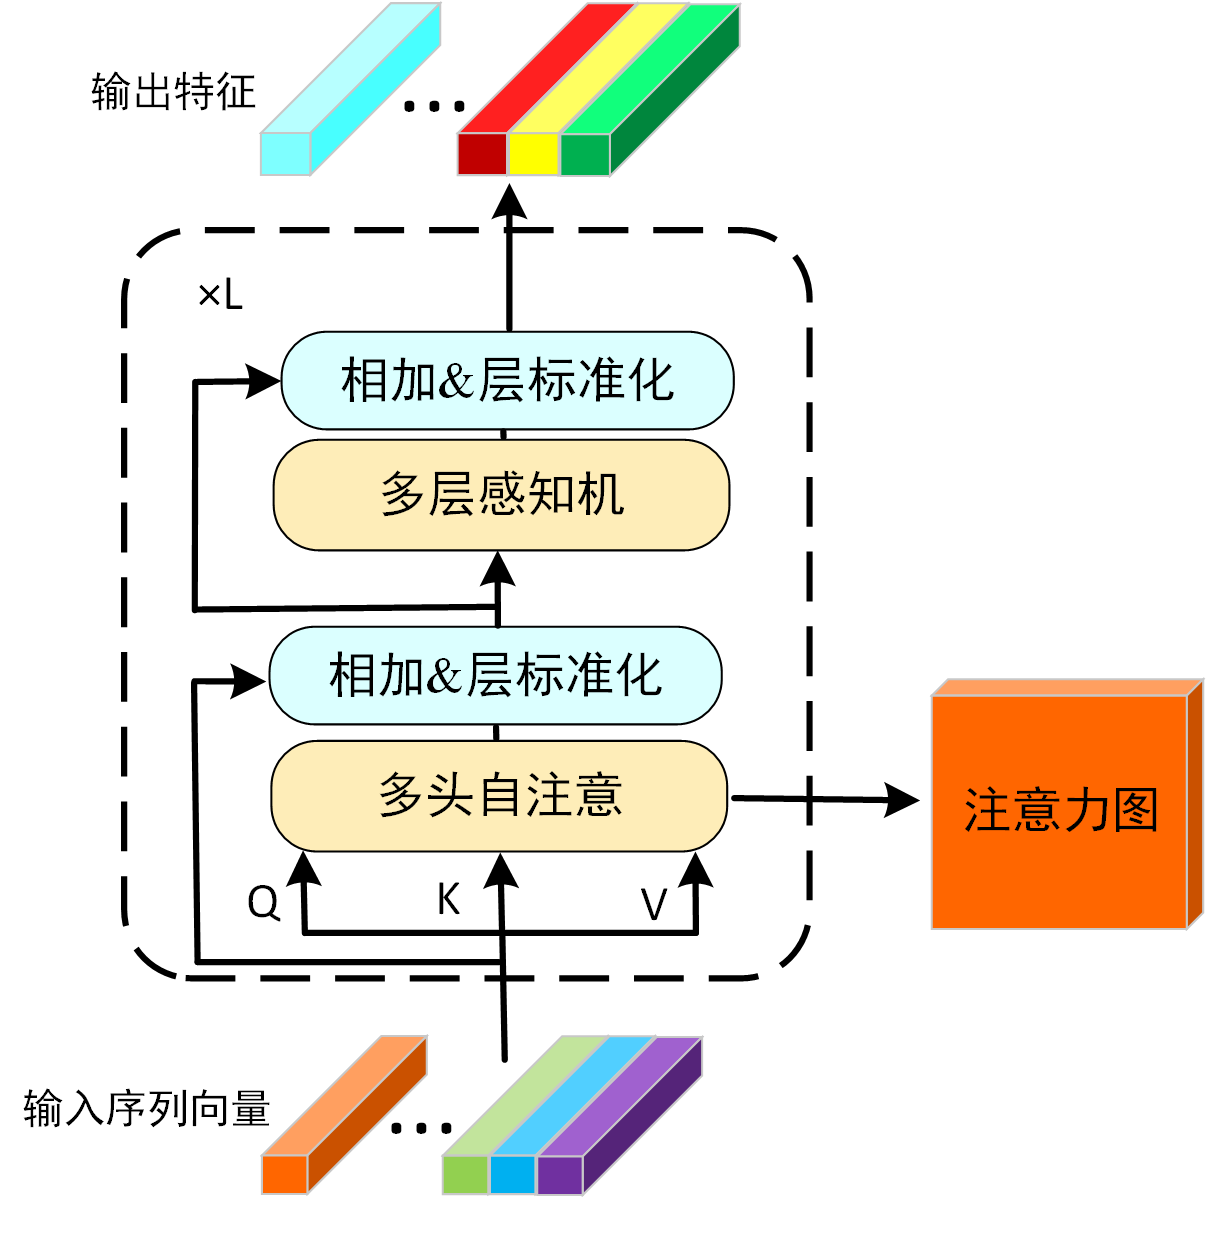
\includegraphics[width=0.65\linewidth]{encoder.png}   
   \caption{Vision Transformer编码模块结构}   
   \label{fig:encoder} 
\end{figure}  

编码模块包含了多头自注意(Multi-head Self-attention,MSA)与多层感知机(Multi-Layer Perceptron, MLP)。
多头自注意模块由$N_h$个单头自注意单元(Self-attention,SA)组成。
对于单头自注意单元,首先将输入$\mathbf{z}_{p} \in \mathbb{R}^{(N+1) \times \mathrm{D}}$,输入经过线性变换得到
查询矩阵$\boldsymbol{Q}$、键矩阵$\boldsymbol{K}$、值矩阵$\boldsymbol{V}$。线性变换如式~\ref{eq:linear}所示:
\begin{equation}
  \begin{array}{ll}
  \boldsymbol{Q}=z_{p} \cdot \boldsymbol{W}^{Q} & \boldsymbol{W}^{Q} \in \mathbb{R}^{\mathrm{D} \times d_{k}} \\
  \boldsymbol{K}=z_{p} \cdot \boldsymbol{W}^{K} & \boldsymbol{W}^{K} \in \mathbb{R}^{\mathrm{D} \times d_{k}} \\
  \boldsymbol{V}=z_{p} \cdot \boldsymbol{W}^{V} & \boldsymbol{W}^{V} \in \mathbb{R}^{\mathrm{D} \times d_{k}}
  \end{array}
  \label{eq:linear}
\end{equation}

其中$d_{k}=\frac{\mathrm{D}}{N_{h}}$ ,得到$\boldsymbol{Q}$、$\boldsymbol{K}$、$\boldsymbol{V}$后,
注意力权重矩阵$\boldsymbol{A}$的计算如式~\ref{eq:attn}所示:
\begin{equation}
  \boldsymbol{A}=\operatorname{softmax}\left(\frac{\boldsymbol{Q} \cdot \boldsymbol{K}^{T}}{\sqrt{d}_{\boldsymbol{k}}}\right), \quad \boldsymbol{A} \in \mathbb{R}^{(N+1) \times(N+1)}
  \label{eq:attn}
\end{equation}

矩阵$\boldsymbol{A}$中的元素$A_{ij}$表示第$i$个特征与第$j$个特征之间的相关性,
值越大则相关性越强,$\sqrt{d_k}$是缩放因子。注意力权重矩阵$\boldsymbol{A}$点乘值矩阵$\boldsymbol{V}$得到单头自注意单元的输出$\mathbf{z}^{\prime}$。
\begin{equation}
  \mathbf{z}^{\prime}=\boldsymbol{A} \cdot \boldsymbol{V}, \quad \mathbf{z}^{\prime} \in \mathbb{R}^{(N+1) \times d_{k}}
  \label{eq:attn_out}
\end{equation}

不同的单头自注意单元在互不干扰、独立的特征子空间中学习相关特征,
最终多头自注意模块对单头自注意单元输出的结果进行拼接,再经过线性变换得到该模块的输出。
该输出与$\mathbf{z}^{\prime}$进行残差连接,经过层标准化(Layer Normalization,LN)作为下一个多层感知机模块的输入。
\begin{equation}
  \operatorname{MSA}\left(\mathbf{z}_{p}\right)=\underset{i \in \mathrm{N}_{\mathrm{h}}}{\operatorname{concat}}\left(\operatorname{SA}\left(\mathbf{z}_{p}^{i}\right)\right) \boldsymbol{W}_{\text {out }}+\boldsymbol{b}_{\text {out }}
  \label{eq:multi_out}
\end{equation}

其中$W_{\text {out }} \in \mathbb{R}^{\mathrm{D} \times \mathrm{D}}$为权重,$\boldsymbol{b}_{\text {out }} \in \mathbb{R}^{(N+1) \times \mathrm{D}}$为偏置。
多层感知机模块由两个全连接层组成,第一个全连接层的激活函数为ReLU,第二个全连接层不使用激活函数,计算公式如下:
\begin{equation}
  \operatorname{MLP}(\boldsymbol{X})=\operatorname{ReLU}\left(\boldsymbol{X} \cdot \boldsymbol{W}_{1}+\boldsymbol{b}_{1}\right) \cdot \boldsymbol{W}_{2}+\boldsymbol{b}_{2}
  \label{eq:msa_out}
\end{equation}

若$\mathbf{z}_{p-1}$为第$p$个编码模块的输入,该编码模块的输出如下式所示:
\begin{equation}
  \begin{array}{l}
  \mathbf{z}_{p}^{\prime}=\operatorname{LN}\left(\operatorname{MSA}\left(\mathbf{z}_{p-1}\right)+\mathbf{z}_{p-1}\right) \\
  \mathbf{z}_{p}=\mathrm{LN}\left(\operatorname{MLP}\left(\mathbf{z}_{p}^{\prime}\right)+\mathbf{z}_{p}^{\prime}\right)
  \end{array}
  \label{eq:encoder_out}
\end{equation}

\subsection{稀疏注意力模块}
血细胞分类中的关键问题是能否准确定位到图像中的辨识性区域,以图~\ref{fig:discriminate}中的粒细胞为例,
不同发育阶段的粒细胞差异较为细微,原始粒细胞与早幼粒细胞染色质都较为细致,区别主要是细胞质中是否存在非特异性颗粒。
中幼粒细胞与晚幼粒细胞染色质都呈现出聚集的索块状,区别主要是细胞核形态是否存在凹陷。
在卷积神经网络中主要通过区域推荐网络或者弱监督的分割掩码来定位图像中的辨识性区域,
而在Vision Transformer模型中,其多头自注意机制可以自主学习不同图像块的权重。
为了充分利用此权重信息实现辨识性区域的定位,本文提出了稀疏注意力模块。
\begin{figure} 
   \centering   
   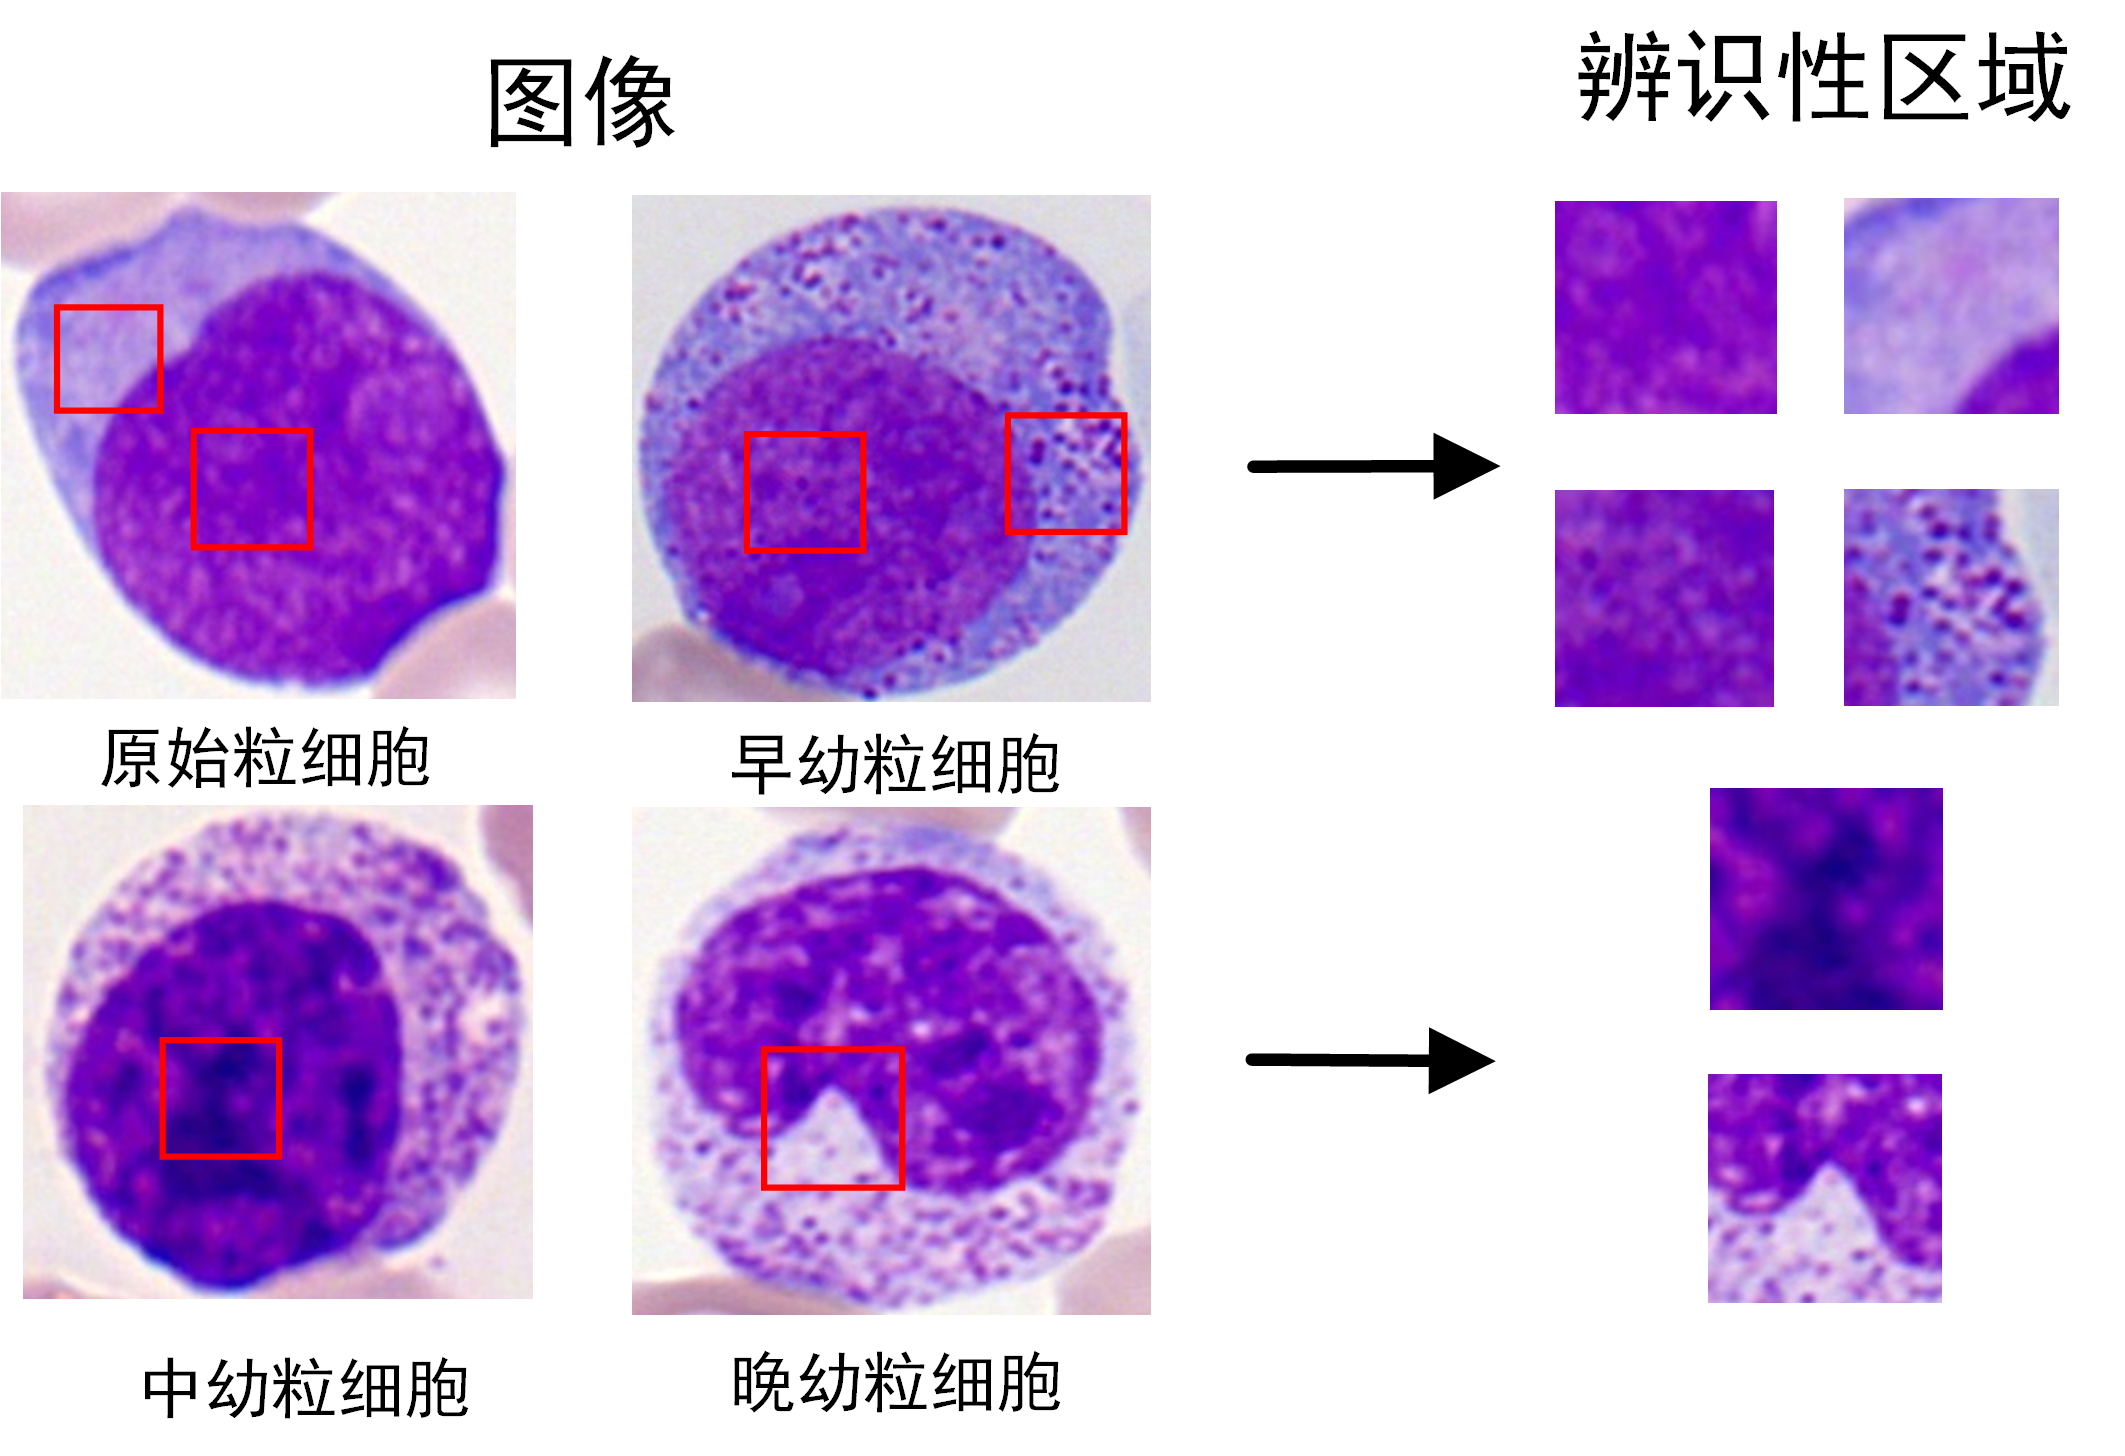
\includegraphics[width=0.7\linewidth]{discriminate.png}   
   \caption{不同类别血细胞的辨识性区域}   
   \label{fig:discriminate} 
\end{figure}  

由于高层次特征的抽象性,其注意力图不一定能代表对应输入图像块的重要性,
因此我们利用先前所有编码模块的注意力图信息并结合压缩激发模块来自主学习每个注意力图的权重。
该模块首先将注意力图全局平均池化为一个描述符,接着使用两个全连接层建模注意力图间的相关性,
最终得到每个注意力图的权重值$\mathbf{\alpha}$。将权重值归一化后与注意力图加权求和得到最终的注意力权重$\boldsymbol{A}_{\mathrm{attn}}$,
如式~\ref{eq:attn_se}所示。整个流程如图~\ref{fig:sparse_attn}所示:
\begin{equation}
  \boldsymbol{A}_{\mathrm{attn}}=\sum_{i=1}^{L-1} \alpha_{i} \boldsymbol{A}_{i}
  \label{eq:attn_se}
\end{equation}

\begin{figure} 
   \centering   
   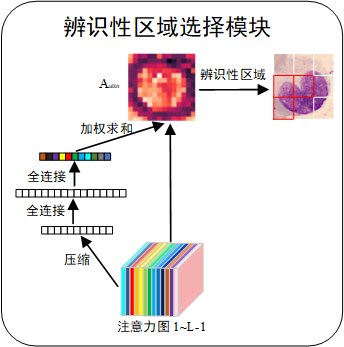
\includegraphics[width=0.60\linewidth]{sparse_attn.png}   
   \caption{稀疏注意力模块结构示意图}   
   \label{fig:sparse_attn} 
\end{figure}  

$\boldsymbol{A}_{\mathrm{attn}}$包含了低层特征与高层特征全部的注意力权重信息,相比于单层的注意力权重$\boldsymbol{A}_{L-1}$更适合筛选辨识性区域。
我们使用$\boldsymbol{A}_{\mathrm{attn}}$中分类向量对应的权重$A_{\mathrm{attn}}^{\text {class }}=\left[\boldsymbol{a}_{\text {final }}^{1}, \boldsymbol{a}_{\text {final }}^{2}, \cdots \boldsymbol{a}_{\text {final }}^{N_{\mathrm{h}}}\right]$,
在$N_h$个自注意头中筛选出最大权重所对应的隐含特征。
最后,将这些隐含特征与分类向量进行拼接作为最后一层编码模块的输入。
\begin{equation}
  \mathbf{z}_{L-1}^{\mathrm{attn}}=\left[\mathbf{z}_{L-1}^{\text {class }} ; z_{L-1}^{a_{1}} ; z_{L-1}^{a_{2}} ; \cdots \mathbf{z}_{L-1}^{a_{N_{h}}}\right]
  \label{eq:attn_se_out}
\end{equation}

稀疏注意力模块将全部序列向量替换为辨识性区域对应的特征向量并与分类向量进行拼接,
然后输入到最后一个编码模块中,这样不仅保留了全局分类特征信息,还强制让最后一个编码层关注到不同类别之间的细微差异部分,
同时舍弃了大量区分度较低的区域信息如背景、超类共同特征等,从而提升了网络的细粒度特征表达能力。

\subsection{损失函数}
像Vision Transformer一样,我们将网络输出的第一个向量即分量向量用于图像分类。\
网络的损失函数包括了交叉熵损失$L_{\text {cross }}$与对比损失$L_{\text {con }}$如式~\ref{eq:loss}所示
\begin{equation}
  L=\left(\boldsymbol{y}, \boldsymbol{y}^{\prime}\right)+L_{\text {con }}(\mathbf{z})
  \label{eq:loss}
\end{equation}

交叉熵损失用于衡量真实标签$\boldsymbol{y}$与网络预测标签的$\boldsymbol{y}^{\prime}$的相似性,定义如式~\ref{eq:loss_ce}所示:
\begin{equation}
  L_{\text {cross }}\left(\boldsymbol{y}, \boldsymbol{y}^{\prime}\right)=-\sum_{i=1}^{c} y_{i} \log \left(y_{i}^{\prime}\right)
  \label{eq:loss_ce}
\end{equation}

为了进一步增加网络提取特征的类内相似性与类间差异性,
我们加入了对比损失$L_{\text {con }}$。对比损失使得不同标签对应的分类特征相似度最小,
相同标签的分类特征相似度最大。为了使正负样本均衡,防止损失被简单的负样本(相似度很小的不同类别特征)所支配,
我们引入阈值$t_{\text {con }}$,只有不同类别样本特征的相似度大于$t_{\text {con }}$时才计入到损失中,当输入数据的批大小为$N$时,
对比损失定义如式~\ref{eq:loss_con}所示:
\begin{equation}
  L_{\text {con }}=\frac{1}{N^{2}} \sum_{i=1}^{N}\left[\sum_{j: y_{i}=y_{j}}\left(1-\frac{\mathbf{z}_{i} \cdot \mathbf{z}_{j}}{\left\|\mathbf{z}_{i}\right\|\left\|\mathbf{z}_{j}\right\|}\right)+\sum_{j: y_{i} \neq y_{j}} \max \left(\frac{\mathbf{z}_{i} \cdot \mathbf{z}_{j}}{\left\|\mathbf{z}_{i}\right\|\left\|\mathbf{z}_{j}\right\|}-t_{\text {con }}, 0\right)\right]
  \label{eq:loss_con}
\end{equation}



% \section{基于分级网络的骨髓血细胞识别方法}

\section{实验结果分析}
\subsection{数据集介绍}
实验数据由自邃蓝智能科技 (上海) 公式提供,单细胞图像通过骨髓血细胞检测网络从原图像中裁剪出来,
随后将单细胞图像大小调整为$224 \times 224$。数据集总共包含了11个类别的血细胞,数据集的分布见~\ref{section:dataset}节。

此外我们采用了The Cancer Imaging Archive平台上开源的血细胞形态学数据集(The Munich AML Morphology Dataset, TMAMD)
该数据来自慕尼黑医院2014年至2017年间100位被诊断为急性白血病的患者与100位无血液恶性肿瘤的患者。
数据集包含了15类由专家标记的18635张单细胞图像。由于数据集存在较严重的类别不平衡问题,部分类别的数量小于30使得网络难以有效的进行特征学习。本文只关注了样本数量大于30的十个类别。
在选择的十个类别中,对于数量较多的类别采用随机欠采样减少样本数量,对于数量较少的类别,采用水平、垂直翻转与旋转90°、180°的方式进行数据扩充,
表~\ref{table:tmamd_dataset}为TMAMD数据集的分布情况与数据增强\cite{van2001art}后的样本分布情况。

\begin{table}
  \caption{TMAMD血细胞数据集数据分布情况}   
  \centering 
  \label{table:tmamd_dataset}
  \begin{tabular}{ccccc}
    \toprule[2pt]
    序号 & 血细胞类别名  &  图像数量 & 是否选择 & 数据增强 \\
    \midrule[1.5pt] 
        1 & 分页核嗜中性粒细胞(NGS) & 8484 & √ & 1000  \\ 
        2 & 杆状核嗜中性粒细胞(NGB)  & 109 & √ & 545  \\ 
        3 & 典型淋巴细胞(LYT) & 3937 & √ & 1000  \\ 
        4 & 非典型淋巴细胞(LYA) & 11 & × &   \\ 
        5 & 单核细胞(MON) & 1789 & √ & 1000  \\ 
        6 & 嗜酸性粒细胞(EOS)  & 424 & √ & 848  \\ 
        7 & 嗜碱性粒细胞(BAS) & 79 & √ & 395  \\ 
        8 & 原始粒细胞(MYO) & 3268 & √ & 1000  \\ 
        9 & 早幼粒细胞(PMO) & 70 & √ & 350  \\ 
        10 & 二分裂早幼粒细胞(PMB) & 18 & × &   \\ 
        11 & 中幼粒细胞(MYB) & 42 & √ & 210  \\ 
        12 & 晚幼粒细胞(MMZ) & 15 & × &   \\ 
        13 & 原始单核细胞(MOB) & 26 & × &   \\ 
        14 & 有核红细胞(EBO) & 78 & √ & 390  \\ 
        15 & 破碎细胞(KSC) & 15 & × &   \\ 
        ~ & 总计 & 18365 & ~ & 6738  \\ 
    \bottomrule[2pt]      
  \end{tabular} 
\end{table}


\subsection{实验环境与评价指标}
实验中图像块的大小设置为$16 \times 16$,
滑动窗步长大小为12,式~\ref{eq:loss_con}中的阈值$t_{\text {con }}$大小为$0.4$,批尺寸大小设置为$32$。
我们在Linux操作系统下的NVIDIA GeForce RTX 3090显卡上训练模型。训练使用的深度学习框架为Pytorch 1.10.1,
优化器使用随机梯度下降算法(SGD),动量设置为0.9,权重衰减设置为5e-4,学习率初始化为0.001,在第40、70、90个epoch时变为原来的1/10。
整个训练过程在第100个epoch停止。

为了定量评估分类算法的性能,我们使用五折交叉验证与精确率(Precision)、召回率(Recall)、准确率(Accuracy)等评价指标,定义如式
~\ref{eq:precision_cls}-~\ref{eq:accuracy_cls}所示
\begin{equation}
  \text { Precision }=\frac{T P}{T P+F P}
  \label{eq:precision_cls}
\end{equation}
\begin{equation}
  \text { Recall }=\frac{T P}{T P+F N}
  \label{eq:recall_cls}
\end{equation}
\begin{equation}
  \text { Accuracy }=\frac{T P+T N}{T P+F P+T N+F N}
  \label{eq:accuracy_cls}
\end{equation}

\subsection{实验结果}

本文方法在慕尼黑TMAMD数据集上各类精确率与召回率如表~\ref{table:cell_tmamd}所示,混淆矩阵如图~\ref{fig:cls_confuse}所示。网络的top-1平均分类准确率为$91.96\%$,
top-5平均分类正确率为$99.48\%$。我们注意到对于最常见的血细胞类型,例如分叶核、杆状核嗜中性粒细胞、典型的淋巴细胞、
嗜酸性粒细胞、有核红细胞,网络预测结果与医生标注达到了极好的一致性,精确率与召回率均高于$90\%$。
而其他类别例如不同发育阶段的粒细胞以及嗜碱性粒细胞,由于相邻发育阶段的粒细胞差异较为细微并且原始样本数量较少,识别更具挑战性,
存在误分类是可以容忍的。
\begin{table}
  \caption{改进Vision Transformer方法的识别精确率与召回率}   
  \centering 
  \label{table:cell_tmamd}
  \begin{tabular}{ccccc}
    \toprule[2pt]
    序号 & 血细胞类别名  &  精确率(\%) & 召回率\%) & 测试图像数量 \\
    \midrule[1.5pt] 
    1  & 嗜碱性粒细胞(BAS)      & 90.41 & 82.50 & 80 \\ 
    2  & 有核红细胞(EBO)        & 98.77 & 100.00 & 80   \\ 
    3  & 嗜酸性粒细胞(EOS)      & 98.81 & 97.65 & 170   \\ 
    4  & 典型淋巴细胞(LYT)      & 94.09 & 95.50 & 200   \\ 
    5  & 单核细胞(MON)          & 86.57 & 93.50 & 200   \\ 
    6  & 中幼粒细胞(MYB)        & 92.31 & 53.33 & 45  \\ 
    7  & 原始粒细胞(MYO)        & 91.50 & 91.50 & 200   \\ 
    8  & 杆状核嗜中性粒细胞(NGB) & 91.82 & 91.81 & 110   \\ 
    9  & 杆状核嗜中性粒细胞(NGB) & 93.50 & 93.50 & 200   \\  
    10 & 早幼粒细胞(PMO)        & 76.92 & 85.71 & 70  \\  
       & 总计                    &      &     & 1355   \\  
    \bottomrule[2pt]      
  \end{tabular} 
\end{table}

\begin{figure} 
   \centering   
   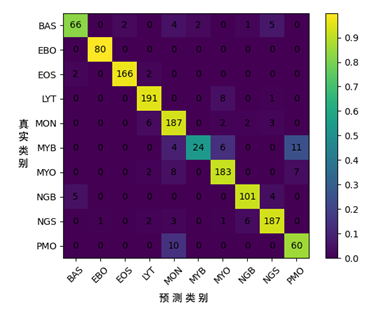
\includegraphics[width=0.75\linewidth]{cls_confuse.png}   
   \caption{改进Vision Transformer的识别混淆矩阵}   
   \label{fig:cls_confuse} 
\end{figure}  

此外,我们将本文提出的方法与其他深度学习方法例如VGG\cite{2014Very}、ResNet\cite{he2016deep}、SE-ResNet\cite{hu2018squeeze}、ResNext\cite{xie2017aggregated}、
EfficientNet\cite{tan2019efficientnet}、Vision Transformer\cite{dosovitskiy2020image}进行了对比。
表~\ref{table:cell_con}为不同方法在TMAMD数据集上的识别结果,表~\ref{table:cell_con}第三列结果表明我们的方法在TMAMD数据上的识别准确率优于其他的方法,取得了有竞争力的性能。
具体而言,我们改进的Vision Transformer与卷积神经网络相比识别准确率提升了$1.5\% \sim 3.0\%$,本文图像块非重叠的模型与其基础框架相比识别准确率提升了$0.74\%$,
而模型的浮点运算次数仅增加$0.09$GFLOPS、参数量增加$7.08$MB。

\begin{table}
  \caption{不同识别方法性能对比}   
  \centering 
  \label{table:cell_con}
  \begin{tabular}{ccccc}
    \toprule[2pt]
    方法 & 骨干网络  &  \makecell{准确率 \\(\%)} & \makecell{运算次数 \\(GFLOPs)} & \makecell{参数量大小\\(MB)} \\
    \midrule[1.5pt] 
    VGG                & VGG16             & 88.85 & 15.53 & 134.31 \\
    ResNet             & ResNet50          & 89.01 & 4.12  & 23.53  \\
    ResNet             & ResNet152         & 89.22 & 11.58 & 78.63  \\
    SENet              & SE-ResNet50       & 89.88 & 4.13  & 26.06  \\
    SENet              & SE-ResNet101      & 89.96 & 7.86  & 47.3   \\
    ResNext            & ResNext50         & 89.22 & 4.27  & 23.00  \\
    ResNext            & ResNext152        & 90.25 & 11.80 & 57.92  \\
    EfficientNet       & EfficientNet-B0   & 90.47 & 0.04  & 19.34  \\
    \hline
    Vision Transformer & vit-base-p16      & 91.14 & 16.86 & 85.81  \\
    本文方法(图像块非重叠)       & vit-base-cell-p16 & 91.88 & 16.95 & 92.89  \\
    本文方法(图像块重叠)        & vit-base-cell-p16 & 91.96 & 19.44 & 92.92\\ 
    \bottomrule[2pt]      
  \end{tabular} 
\end{table}

图~\ref{fig:self_attn}中展示了本文模型的自注意力图。我们在数据集中随机选取了八个血细胞(细胞1-细胞8),其中,第一列为原始图像,
第二列为整合后的注意力图,每种颜色表示不同头部的注意力。第三到八列为稀疏注意力模块多头注意力单元前六个头部所对应的注意力图。
从整合注意力图中我们可以看到,细胞核、细胞质与背景分别被不同头部标记为不同的颜色。因此,本文模型的自注意机制有能力区分目标的不同区域。
此外,我们将稀疏注意力模块每个头部最大权重对应的图像块进行标记,如图~\ref{fig:sparse_select}所示。第一行图像中的红色边框为稀疏注意力模块所挑选的图像块区域,
第二行为整体注意力图。我们看到模型主要关注了细胞核与细胞质等辨识性区域。以上可视化结果表明,本文模型成功捕捉到了细胞中的辨识性区域。
\begin{figure} 
  \centering   
  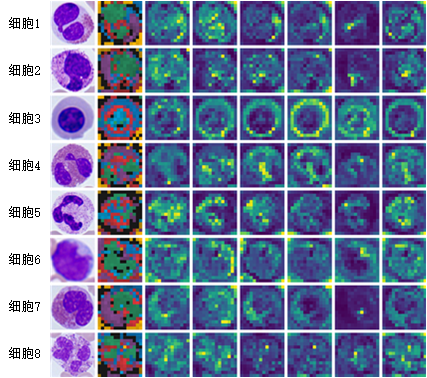
\includegraphics[width=0.85\linewidth]{self_attn.png}   
  \caption{可视化自注意力图}   
  \label{fig:self_attn} 
\end{figure}  

\begin{figure} 
  \centering   
  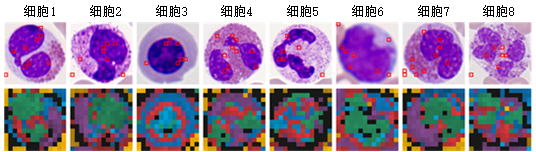
\includegraphics[width=0.95\linewidth]{sparse_select.png}   
  \caption{稀疏注意力模块选择的图像块}   
  \label{fig:sparse_select} 
\end{figure}  

从表~\ref{table:cell_con}中可以看到,本文最优模型的浮点运算次数与参数量大小均大于卷积神经网络方法,
而卷积网络中的EfficientNet模型通过神经架构搜索,具有更优运算次数与识别准确率。
因此,本文进一步探究了Transformer结构中嵌入向量的维度、编码层数量、与多头注意力的头数与模型准确率的关系,
从而找到更好地模型速率与准确率的平衡。我们设计不同的超参数如表~\ref{table:detect_con}所示,编码层数量为$4$、头数量为$4$,嵌入向量维度为$256$时,
模型最小只有7MB,运算次数为1.18GFLOPS,但准确率较低仅有$78.08\%$。
当将编码层的层数从12减少到2层,多头自注意的数量与嵌入向量维度不变时,模型的准确度由$91.88\%$下降到了$83.17\%$。
当编码层数相同时,嵌入向量维度越低,模型的识别准确率也相应降低。整体来说,当本文模型识别准确率高于卷积网络时,参数量与运算次数也高于卷积网络。
未来我们会关注于Transformer网络的结构搜索,从而找到更加精准的模型速率与准确率的平衡。

\begin{table}
  \caption{不同识别方法性能对比}   
  \centering 
  \label{table:detect_con}
  \begin{tabular}{cccccc}
    \toprule[2pt]
    编码层数量 & 多头自注意数 & 嵌入向量维度 &  \makecell{运算次数 \\(GFLOPs)} & \makecell{参数量大小\\(MB)} & \makecell{准确率 \\(\%)} \\
    \midrule[1.5pt] 
        12 & 12 & 768 & 16.95 & 92.89 & 91.88 \\
        10 & 12 & 768 & 14.16 & 78.73 & 90.85  \\
        8 & 12 & 786 & 11.37 & 64.54 & 89.81  \\
        6 & 12 & 768 & 8.58 & 50.37 & 87.64 \\
        4 & 12 & 768 & 5.79 & 36.28 & 85.01  \\
        2 & 12 & 768 & 3.0 & 22.02 & 83.17 \\
        12 & 8 & 512 & 10.04 & 55.13 & 84.12 \\ 
        8 & 8 & 512 & 6.73 & 38.32 & 82.41 \\
        4 & 8 & 512 & 2.8 & 17.57 & 80.85  \\
        12 & 4 & 256 & 4.39 & 24.18 & 78.64 \\
    \bottomrule[2pt]      
  \end{tabular} 
\end{table}

\subsection{消融实验}
我们将本文模型进行消融实验研究来分析不同模块对细胞图像识别的影响,
我们分别评估了图像块的划分方法,稀疏注意力模块,对比损失的影响。

\subsubsection{图像块划分方法}
我们探究了图像块划分大小与图像块是否重叠对模型识别准确率的影响,实验结果如表~\ref{table:split_method}所示。、
图像块大小为32相比于大小为16的划分方式,嵌入后向量数量与模型的计算量都大幅降低,训练与推理的时间也减少约3/4,
但是模型的识别准确率较差。无论块大小是16还是32,重叠划分方式相比非重叠划分方式模型识别准确率均有提高,
而由此引入的额外计算成本也是可以接受的。图~\ref{fig:split_method}实验结果表明,图像块划分越小,
图像块之间存在重叠可以使得图像的局部细节保留的更加完整,模型的识别准确率越高。

\begin{table}
  \caption{不同图像块划分方式的消融研究}   
  \centering 
  \label{table:split_method}
  \begin{tabular}{cccccc}
    \toprule[2pt]
    块大小 & 划分方式 & 嵌入向量数量 & \makecell{准确率 \\(\%)} & \makecell{运算次数 \\(GFLOPs)}\\
    \midrule[1.5pt] 
        32 & 非重叠 & 50 & 88.92 & 4.36  \\ 
        32 & 重叠 & 82 & 89.88 & 7.16  \\ 
        16 & 非重叠 & 197 & 91.88 & 16.95  \\ 
        16 & 重叠 & 226 & 91.96 & 19.44  \\ 
    \bottomrule[2pt]      
  \end{tabular} 
\end{table}
\begin{figure} 
  \centering   
  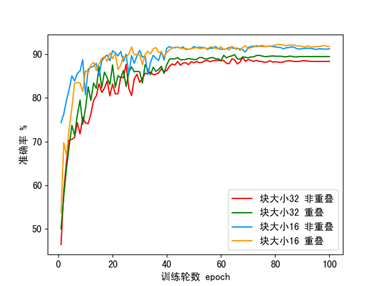
\includegraphics[width=0.7\linewidth]{split_method.png}   
  \caption{图像块划分方式对模型性能的影响}   
  \label{fig:split_method} 
\end{figure}  

\subsubsection{稀疏注意力模块}
通过稀疏注意力模块来选择显著性图像块作为最后编码层的输入,模型的识别准确率从$91.14\%$ 
提高到$91.8\%$。我们认为通过稀疏注意力的方式,模型将采样最具辨别力的图像块作为输入,
从而明确丢弃一些无用的图像块并迫使网络对重要的部分进行学习。

\subsubsection{对比损失}
Vision Transformer与本文模型在有无对比损失情况下的识别性能如表~\ref{table:con_loss}所示。实验结果表明,通过加入对比损失,Vision Transformer的识别准确率提升了$0.52\%$,
本文模型的识别准确率提升了$0.59\%$。图~\ref{fig:tsne}为测试集图像与本文模型输出分类特征的t-SNE\cite{van2008visualizing}降维可视化结果,
我们发现加入对比损失后,不同类别的分类特征在嵌入到二维空间后距离增大,相同类别的分类特征距离减小。
综合上述结果,我们认为加入对比损失可有效扩大相似子类之间的特征距离,并减少相同类别之间的特征距离,从而提升模型的识别性能。

\begin{table}
  \caption{对比损失的消融研究}   
  \centering 
  \label{table:con_loss}
  \begin{tabular}{ccc}
    \toprule[2pt]
    方法 & 对比损失 & \makecell{准确率 \\(\%)} \\
    \midrule[1.5pt] 
        Vision Transformer & × & 90.62  \\ 
        Vision Transformer & √ & 91.14  \\ 
        本文模型 & × & 91.29  \\ 
        本文模型 & √ & 91.88  \\ 
    \bottomrule[2pt]      
  \end{tabular} 
\end{table}

\begin{figure}[htbp]
	\centering
  \begin{subfigure}{0.45\linewidth}
    \centering
    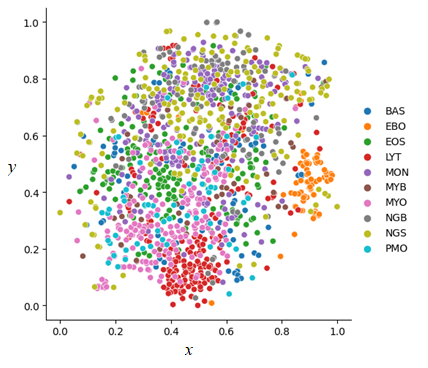
\includegraphics[width=0.95\linewidth, height=0.81\linewidth]{tsne1.png}
    \caption{测试集图像t-SNE降维}
  \end{subfigure}
  \\
	\centering
	\begin{subfigure}{0.45\linewidth}
		\centering
		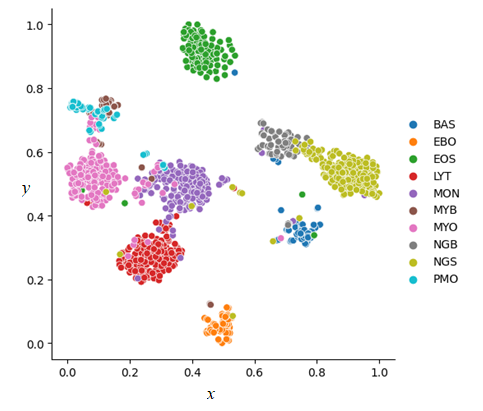
\includegraphics[width=0.95\linewidth, height=0.81\linewidth]{tsne2.png}
    \caption{无对比损失分类特征t-SNE降维}
	\end{subfigure}
	\centering
	\begin{subfigure}{0.45\linewidth}
		\centering
		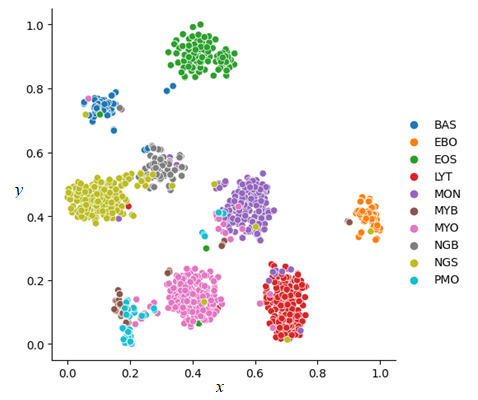
\includegraphics[width=0.95\linewidth, height=0.81\linewidth]{tsne3.png}
    \caption{使用对比损失分类特征t-SNE降维}
	\end{subfigure}
  \caption{t-SNE降维可视化结果}
	\label{fig:tsne}
\end{figure}

% \subsection{分级网络性能分析}

\section{小结}
目前血细胞识别研究主要侧重于五类血细胞的粗分类,很少有研究关注血细胞大类中子类的识别。
针对上述问题,本章提出了一种基于改进Vision Transformer的血细胞识别模型。
我们基于Vision Transformer中的自注意机制提出了稀疏注意力模块,该模块综合利用了所有编码层的注意力权重信息,
捕捉到图像中的辨识性区域,提升了模型的细粒度特征表达能力。
本文采用对比损失进一步增加了网络学习特征的类内一致性与类间差异性。
本文方法在TMAMD数据集上取得了先进的性能,定性与定量的可视化结果均表明了本方法的有效性与可解释性。
相较于其他识别方法,本文方法具有更高的识别准确率,有望为医生临床诊断提供参考依据,具有潜在的临床应用前景。